\section{Caso 3. Dos fuentes de datos donde una es externa y dos ontologías}

Se pretende demostrar la integración e interoperabilidad con una ontología específica y una genérica. Para esto, se utilizaron los datos de Procesos Licitatorios de la DNCP junto con la ontología OCDS, y también los datos disponibles en Wikidata junto con su ontología propia. Con esto se enriqueció la fuente de datos primaria a partir de una fuente de datos externa, la cual permitió obtener más información relevante y contextual.

La consulta realizada en el cuadro xx consiste en obtener la cantidad de todos los Procesos Licitatorios cuyos proveedores residen en países que no son limítrofes con Paraguay, agrupando estas cantidades de acuerdo al país.


\begin{lstlisting}[captionpos=b, caption=Información referente al proceso licitatorio cuyo identificacor es, label=lst:caso1,  numbers=left,  numberstyle=\tiny\color{mygray},
    basicstyle=\ttfamily,frame=single]
select *
    where {
      {
      select ?label (COUNT(?label) AS ?cantidad)
    where {
    ?plicitatorio rdf:type ocds:Release;
                  ocds:contracts ?contract.
      ?contract ocds:contractSuppliers ?org.
      ?org ocds:address ?b .
    ?b ocds:countryName ?label
          MINUS  { SERVICE <https://query.wikidata.org/sparql>
                        { 
        SELECT DISTINCT  (str(?labelWhitLang) as ?label)
            WHERE
                { wd:Q733   wdt:P47    ?paislimitrofe .
                
                    ?paislimitrofe wdt:P297    ?codigoPais.
                            ?paislimitrofe     rdfs:label ?labelWhitLang. 
                    FILTER (langMatches( lang(?labelWhitLang), "ES" ) )
                }        
        }
        }
        } group by ?label
      }
    
    }
 \end{lstlisting}

 Primeramente se seleccionan todos los Procesos Licitatorios junto con el país donde residen (ocds:countryName) excluyendo (MINUS) todos los países que sean limítrofes con Paraguay. En Wikidata, wd:Q733 es el identificador de país de Paraguay mientras que wdt:P47 es el identificador de la propiedad “comparte frontera con” y rdf:label es el nombre de país. El comando SERVICE nos permite realizar consultas a otro punto Sparql, en este caso Wikidata. La única información necesaria para lograr este enlace es conocer la URI que representa el Punto Sparql para así poder realizar consultas sobre los datos externos.


Se utilizó el nombre del país en ambos conjuntos de datos como elemento de relación entre países para conseguir suprimir del resultado los países que son limítrofes con Paraguay. Se tomó la decisión de utilizar este atributo debido a que no hay una relación directa entre un país en el conjunto de datos de la DNCP y el mismo país en el conjunto de datos de Wikidata. En la imagen xx se muestran los resultados obtenidos.


\begin{figure}[h!]
    \centering
    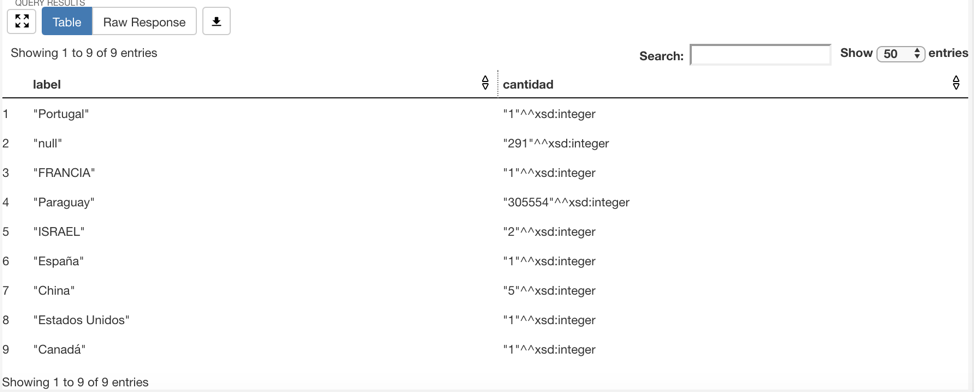
\includegraphics[width=150mm]{figuras/caso3Resultado1.png}
    \caption{Despliegue de resultado de la consulta del caso 3}
    \label{img:caso1Resultado}
 \end{figure}


En la figura xx se ve el resultado si se suprime el filtro por países limítrofes correspondientes a las líneas desde la xx a la xx. En la figura xx se presenta un diagrama de relaciones entre las dos fuentes de datos, las ontologías utilizadas y la consulta.


 \begin{figure}[h!]
    \centering
    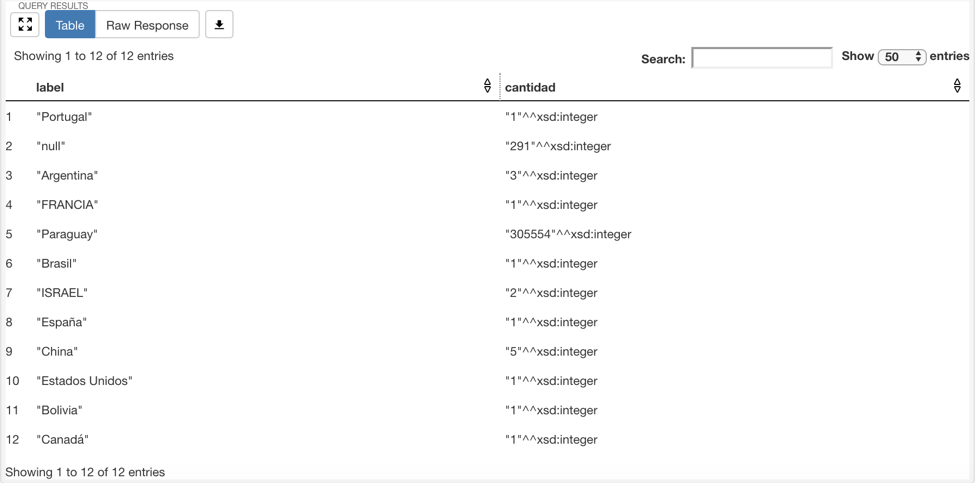
\includegraphics[width=150mm]{figuras/caso3Resultado2.png}
    \caption{Despliegue de resultado de la consulta del caso 3}
    \label{img:caso1Resultado}
 \end{figure}


 \begin{figure}[h!]
    \centering
    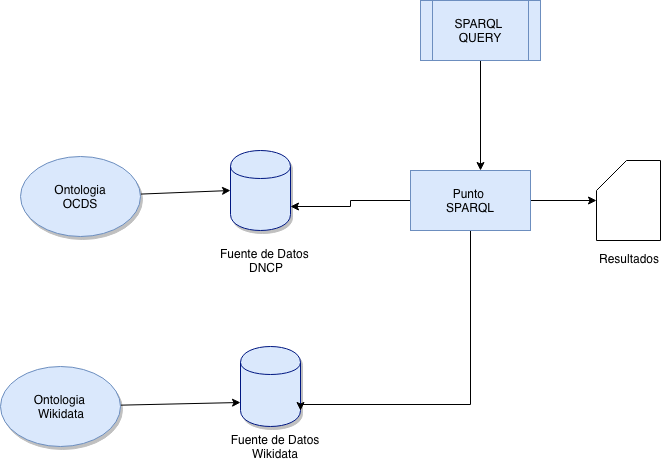
\includegraphics[width=150mm]{figuras/Diagramas-Caso 3.png}
    \caption{Despliegue de resultado de la consulta del caso 3}
    \label{img:caso1Resultado}
 \end{figure}

 Esta consulta podría tener inconvenientes si la forma de escribir del nombre de los país cambiara, es el caso de ISRAEL en la línea 5 de la figura xx que se encuentra en mayúsculas. Para evitar esto, lo óptimo sería que los atributos no sean de tipo texto sino más bien sean objetos dentro del conjunto de datos de la DNCP y éstos estén relacionados con otros semejantes dentro de la Web Semántica.

En el cuadro xx se muestra la definición actual de la propiedad “countryName” que pertenece a la clase “Address". Se observa que el tipo de propiedad es “DatatypeProperty” el cual representa un literal. 

\begin{lstlisting}[captionpos=b, caption=Información referente al proceso licitatorio cuyo identificacor es, label=lst:caso1,  numbers=left,  numberstyle=\tiny\color{mygray},
    basicstyle=\small,frame=single]
###  http://purl.org/onto-ocds/ocds#countryName
:countryName rdf:type owl:DatatypeProperty ,
    owl:FunctionalProperty ;
    rdfs:domain :Address ;
    rdfs:range xsd:string ;
    rdfs:comment "The country name. For example, United States."@en ;
    rdfs:label "Country name"@en .
 \end{lstlisting}


 En el cuadro xx se muestra una posible solución al inconveniente mencionado. Primeramente se debe renombrar la propiedad “countryName” a “country” para que de esta forma denote la relación con un país y no con el nombre del país solamente. Luego se debe cambiar el rango de valores de “rdfs: range xsd:string” a “rdfs:range :Country” donde “Country” se refiere a una nueva clase a ser definida en la ontología. Esta última será la que represente al concepto “País”. Luego deberá definirse una instancia del país (por cada país que exista en la fuente de datos) de tipo “Country”. Finalmente faltaría relacionar este recurso con otro semejante dentro de la Web Semántica, en este caso se puede realizar con los datos disponibles en Wikidata a través de la sentencia “owl:sameAs wd:Q733” donde “wd:Q733” es el identificador único (URI) de Paraguay en Wikidata.

 \begin{lstlisting}[captionpos=b, caption=Información referente al proceso licitatorio cuyo identificacor es, label=lst:caso1,  numbers=left,  numberstyle=\tiny\color{mygray},
    basicstyle=\small,frame=single]
PREFIX wd: <http://www.wikidata.org/entity/>

###  http://purl.org/onto-ocds/ocds#country
:country rdf:type owl:ObjectProperty ,
                      owl:FunctionalProperty ;
             rdfs:domain :Address ;
             rdfs:range :Country ;
             rdfs:comment "El pais donde reside"@es ;
             rdfs:label "Pais de residencia"@en .

###  http://purl.org/onto-ocds/ocds#Country
:Country rdf:type owl:Class ;
         rdfs:comment "Representa un pais."@es ;
         rdfs:label "Pais"@es .

###  http://purl.org/onto-ocds/ocds#countryParaguay
:countryParaguay rdf:type owl:NamedIndividual ,
                                    :Country ;
                           dcterms:title "Republica del Paraguay"@es ;
                           rdfs:label "Paraguay"@es .
    owl:sameAs wd:Q733
 \end{lstlisting}

